% \section{Energy benchmarking}

% \TODO{Armstrong}

% \begin{itemize}
% \item What kind of tools and framework exist to measure all these metrcis? What literature exist that have addressed energy measurement?
% \item Can we as scientist create our own PUE?
% \item XX \url{https://codecarbon.io/}
% \item Create a survey study to include a generalized framework above one particular 
% \item Cite Gregor Von Laszewski's ppers: \url{https://ieeexplore.ieee.org/document/5493462}
% \item plot a TDP/Core-count Y-axis aganst x-time
% \item Use python matplotlib to show different CPU's/GPUs TDP/Core over time scattered plot
% \item FLOPS 32, we can add FLOPS 64 
%     - Add more rows in the table
% \url{https://top500.org/lists/top500/2024/11/}
% \item What are the most important energy measurement for program
% \item what are the most important bennchmarks for power consumptions in data center?
% \url{https://arxiv.org/html/2410.12032v1}
% \end{itemize}

% \subsection{Introduction and Importance}
% \textcolor{red}{Written by K Mirza}
% Energy consumption has quickly become a critical dimension of machine learning benchmarking. Training and deploying modern AI systems can require enormous computational resources, often rivaling the annual energy consumption of households. Training a single large-scale language model can consume megawatt-hours of electricity. GPT-3 took roughly 1287 MWh to train \cite{en18174701}, this is roughly equivalent to the annual power consumption of 130 homes in the US \cite{WECEnergy}. More traditional benchmarks such as FLOPS or latency provide performance insights but overlook 'energy-to-solution' which measures the total energy required to complete a task. Without perspective researchers and practitioners risk optimizing for speed at the expense of sustainability and cost efficiency.  

% Energy benchmarking address this gap by:
% \begin{itemize}
%     \item Quantifying the environmental footprint of AI workloads (carbon emissions, renewable vs. non-renewable energy use).
%     \item Highlighting economic tradeoffs in large-scale computing (cloud costs, datacenter efficiency). 
%     \item Guiding hardware and algorithmic choices towards a more effective architecture. 
%     \item Supporting policy and funding decisions by providing transparent data on sustainability. 
% \end{itemize}
% Energy aware benchmarks help ensure that AI development aligns with broader goals of responsible computing making results reproducible, performant, economically and environmentally sustainable. 

% \subsection{Measurements}

% \paragraph{Temperature.}

% \paragraph{Total Energy.}

% \paragraph{PUE.}

% Power Usage Effectiveness. 
% A metric commonly used to measure the energy efficiency of data centers.

% PUE is defined as:

% \[PUE= \frac{Energy~Usage~of~IT~Equipment}
%             {Total~Facility~Energy~Usage}
% \]

% DCiE = 


%  \paragraph{Green500}

% \paragraph{MLCommons}

% Who does energy, i think tiny does, who else

% \paragraph{Carbon Footprint.}

% \subsection{Tradeoffs}

% Turbo mode

% \subsection{Economic Impact}

% \subsection{Environmental Impact.}


% \paragraph{Energy Sources.}

% \paragraph{Carbon credits.}

% \paragraph{Energy Consumption.}

% \paragraph{Geographical Diversity.}

% \subsubsection{Energy Measurement Tools and Measurement Frameworks}

% \subsection{Tools}


% \begin{itemize}
%     \item temperature benchmarking
%     \item Basic energy concepts, total energy footprint, PUE
%     \item Carbon footprint
%     \item Tax Credits
%     \item Renewable resources
%     \item geographical diversity
% \end{itemize}

% %================================ ENERGY ===============================
% \section{Energy Benchmarking}
% \label{sec:energy}
% \TODO{Armstrong}

% The recent wave of exascale procurements, the rise of trillion-parameter
% language models, and net-zero pledges by hyperscale cloud providers have
% elevated \emph{energy-to-solution} from a niche afterthought to a primary
% design constraint for both HPC and AI systems. In what follows, we
% consolidate the landscape of energy-aware benchmarks and tools
% (Table~\ref{tab:hpc_energy_catalog}), survey state-of-the-art measurement
% toolchains, and outline an experimental blueprint that scientific 
% consortia, such as the MLCommons Science Working Group, can adopt to
% conduct reproducible, large-scale studies of energy efficiency.

% %---------------------------------------------------------------------
% \subsection{From ``How Fast?'' to ``How Fast per Joule—and at What Climate Cost?''}
% \label{sec:energy:bg}

% Benchmarks such as \textbf{Green500} (\(\mathrm{GFLOPS/W}\)) and
% \textbf{MLPerf Power} (J/sample) have become de-facto compass points for
% hardware road-maps and even procurement RFPs~\cite{Scogland11Green500,Tschand24MLPerfPower}. At chip scale,
% dynamic-voltage–frequency scaling (DVFS) or mixed-precision kernels can
% double or triple runtime yet deliver up to a ten-fold gain in joules per
% operation \cite{Peon23A100PowerCap}. On the facility side, a
% \(\pm\)10 ¢ kWh\(^{-1}\) swing can tip the ROI between air and liquid
% cooling and alter the attractiveness of renewable PPAs
% \cite{Koomey21HyperscaleCost}. The effect is visible in the November 2024 and June 2025 Green500 list, where the \emph{JEDI prototype\footnote{\url{https://top500.org/lists/green500/2025/06/}}}  consecutively tops the chart at 72.73 GFLOPS/W~\cite{Green500Nov2024}. Consequently, recent literature frames the key question as ``how fast \emph{per joule} and \emph{per kg CO\(_2\)e}''~\cite{Scogland11Green500,NVIDIA23Blog,Tschand24MLPerfPower}.

% \subsubsection*{Energy-Aware Benchmarks and Tooling representations}
% The advanced of energy benchmarking spans the compute continuum—from
% enterprise servers through exascale systems down to micro-controllers—and
% offers metrics at three distinct layers:

% \begin{itemize}
%     \item \textbf{Head-line benchmark suites} quantify whole-system
%           efficiency.  Examples include SPECpower\_ssj2008
%           (watts\;/transaction), TPC-Energy and JouleSort
%           (watt-hours\;/DB phase or records\;/joule), Green500,
%           HPCG-Power and HPL-MxP (GFLOPS\;/W), plus MLPerf Power and
%           MLPerf Tiny (joules\;/epoch or {\textmu}J\;/inference).  Their
%           scores guide procurement, regulatory compliance (ENERGY STAR,
%           EU Lot 9) and public leaderboards.

%     \item \textbf{Instrumentation frameworks} stream calibrated power
%           traces at node, container, or function scope.  PTDaemon anchors
%           external-meter calibration; Scaphandre, Kepler, IBM PowerAPI
%           and NVIDIA DCGM Energy expose RAPL/NVML feeds to Prometheus;
%           Intel VTune Power and Cray PAT Energy Counters drill down to
%           per-kernel joules.  These data streams feed power-aware
%           schedulers, autotuners, and job-level carbon dashboards.

%     \item \textbf{Domain-specific mini-apps and wrappers} bridge
%           performance and climate impact.  Mini-app “Power’’ add-ons
%           (LULESH, ExaSMR, CosmoFlow, DeepCAM, GROMACS-EE, etc.) let researchers explore DVFS and precision trade-offs without
%           porting full production codes, while wrappers such as
%           CodeCarbon and CarbonTracker translate kilowatt-hours into
%           real-time kg CO\(_2\)e via grid-intensity APIs.
% \end{itemize}

% Collectively, these efforts provide levers that range from joules-per-instruction optimization at the chip level, through job-level Energy–Delay Product tuning, up to fleet-scale sustainability audits expressed in PUE and
% kg $CO_2$e. Thus, ensuring that energy efficiency is treated as a first-class metric alongside raw performance.


% 
\begin{table*}[hptb]
  \centering
  \caption{
  Energy- or carbon-efficiency benchmarks (B) and tools (T) used in scientific-HPC research.  Metrics use ``/'' for ``per''; ``;'' separates multiple items; ``+'' appears only where a spec explicitly combines two values into one score
  %Benchmarks, tools, and initiatives that publish energy‑ or carbon‑efficiency metrics for Scientific‑HPC workloads.
  }
  \label{tab:hpc_energy_catalog}
  %\renewcommand{\arraystretch}{1.1}
  %\setlength{\tabcolsep}{4pt}
  \rowcolors{2}{white}{lightgray}
  \begin{tabularx}{1.0\textwidth}{|llllX|}
    \toprule
    & \headerfont\textbf{(B)enchmark or (T)ool}
    & 
    & \headerfont\textbf{Core metric(s) } %\& data captured} 
    & \headerfont\textbf{Typical Benchmarking Use}\\ 
    \midrule
B & SPECpower\_ssj2008           & \cite{specpower}            & W/transaction; ops/W                & Enterprise-server rankings; ENERGY STAR compliance \\
B & SPEC\,SERT$^{2}$             & \cite{sert2}                & Server-Efficiency-Rating = kWh + perf    & EU Lot 9 certification; vendor datasheets \\
B & TPC-Energy                   & \cite{tpcenergy}            & Wh/DB phase                            & OLTP/warehouse energy cost studies \\
B & JouleSort                    & \cite{joulesort}            & records/J                              & Storage-I/O contests; I/O-stack tuning \\
B & Green500                     & \cite{green500}             & GFLOPS/W (HPL or HPL-AI)               & Global supercomputer energy ranking \\
B & HPCG-Power                   & \cite{hpcgpower}            & GFLOPS/W (HPCG)                        & Memory-bound tuning; procurement add-on to TOP500 \\
B & HPL-MxP (HPL-AI)             & \cite{hplmxphplai}          & mixed-precision GFLOPS/W               & GPU/TPU evaluation for AI-optimised LINPACK \\
B & MLPerf Power                 & \cite{mlperfpower}          & J; avg W; J/sample; J/epoch       & Official energy track for MLPerf submissions \\
B & MLPerf Tiny                  & \cite{mlperftiny}           & $\mu$J/inference (MCU)             & Edge-AI board comparison; ultra-low-power design \\
B & CoreMark-PRO Power           & \cite{coremarkpro}          & iterations/s/W (SoC)                 & Pre-silicon DVFS sweeps; embedded RFPs \\ 
B & UL Procyon AI Power          & \cite{procyon}              & images/W; fps/W                     & Smartphone \& laptop AI-inference benchmarks \\
B & CANDLE Power Study           & \cite{candlepowerstud}      & J/epoch; GFLOPS/W                   & DOE accelerator procurement guidance \\
B & LULESH/miniFE Energy       & \cite{luleshminifeene}      & J/iteration                            & DVFS + autotuning baselines \\
B & ExaSMR Power Benchmark       & \cite{exasmrpowerbenc}      & J/neutron; energy-vs-accuracy curve   & Energy budget strategy in nuclear simulations \\
B & EE-HPC-WG Energy Benchmark   & \cite{eehpcwgenergybe}      & draft node/job spec; JSON trace       & Toward common HPC energy standard \\
B & HPC-AI500 Energy Track       & \cite{hpcai500energyt}      & planned: GFLOPS/W; tokens/J         & Mixed AI/HPC cluster evaluations \\
B & PARSEC-3.1 Energy Extension  & \cite{parsec31energye}      & W; J via PAPI-RAPL; J/op; EDP       & Pre-silicon DVFS research \\
B & CosmoFlow-Power              & \cite{cosmoflow2019}        & J/epoch; GFLOPS/W                   & CNN scaling on 15 k+ GPUs \\
B & HACC Energy Add-on           & \cite{hacc2020power}        & J/particle update                      & N-body cosmology power studies \\
B & DeepCAM-Energy               & \cite{deepcam2020power}     & J/epoch (UNet)                         & Climate-analytics accelerator studies \\
B & OpenIFS-Energy               & \cite{openifsenergy2023}    & kWh/model-day; W timeline             & Weather-model node comparison \\
B & GROMACS-EE                   & \cite{gromacsee2024}        & J/ns; W/GPU                         & MD clock-vs-accuracy trade-offs \\
B & NAMD-Power                   & \cite{namdpower2019}        & Energy-Delay-Product (ApoA1)             & Summit node DVFS optimisation \\
B & QE Energy Suite              & \cite{qeenergy2022}         & J/SCF step; GFLOPS/W                & DFT GPU-offload studies \\
B & VASP-Power Harness           & \cite{vasppower2023}        & W; kWh/MD step                        & Materials-science accelerator compare \\
B & OpenFOAM-Energy              & \cite{openfoamenergy2021}   & J/1k iterations                       & CFD partitioning \& mesh tuning \\
B & InSAR-AI Power Kit           & \cite{insarpower2024}       & J/satellite scene                      & Edge-to-cloud EO inference cost \\
B & H3D-Energy                   & \cite{h3denergy2023}        & J/hydrology timestep                & Hydrology model DVFS exploration \\ \hline\hline  
T & PTDaemon/SERT Energy       & \cite{specptdaemonser}      & calibrated W; kWh (node)                & Lab reproducibility; Lot 9 labels \\
T & Scaphandre                   & \cite{scaphandre}           & W; kWh (process/node, Prometheus)     & Slurm dashboards; power-cap feedback \\
T & Kepler                       & \cite{kepler}               & W/pod; J/pod (eBPF)                 & Energy observability in K8s clusters \\
T & CodeCarbon                   & \cite{codecarbon}           & kWh; kg CO\(_2\)e (process)             & Rapid CO\(_2\) estimation in pipelines \\
T & CarbonTracker                & \cite{carbontracker}        & measured + predicted kWh; CO\(_2\)e     & Scheduling DL jobs in low-carbon hours \\
T & PowerPACK/Mont-Blanc       & \cite{powerpackmontbl}      & W; J for MPI/OpenMP mini-apps         & Network-topology \& DVFS studies \\
T & Cray PAT Energy Counters     & \cite{craypatenergyco}      & J/function; avg W                     & Kernel hotspot hunting on Shasta \\
T & IBM PowerAPI (pmlib)         & \cite{ibmpowerapipmli}      & kWh (job/process)                      & Energy-aware scheduling on Summit \\
T & NVIDIA DCGM Energy           & \cite{nvidiadcgmenerg}      & W; J (GPU) \@ 1Hz; telemetry           & GPU power-cap discovery; Green500 \\
T & Intel VTune Power            & \cite{intelvtunepower}      & package W; J/function                 & Roofline-vs-energy tuning on Xeon \\ 

\bottomrule   
  \end{tabularx}
\end{table*}


 
 
 %  B & SPECpower\_ssj2008 & \cite{specpower}            & Watts per transaction; ops/W & Enterprise‑server energy rankings and ENERGY STAR compliance \\  
 % B  & SPEC SERT$^{2}$  & \cite{sert2}                   & Server Efficiency Rating (kWh+perf)& Lot 9 regulatory testing; vendor datasheets \\  
 % B  & TPC‑Energy  & \cite{tpcenergy}                    & Watt‑hours per database phase & Energy‑cost analysis for OLTP/warehousing appliances \\  
 % B  & JouleSort  & \cite{joulesort}                     & Records per Joule  B  & Storage‑I/O hardware contests; I/O stack optimisation \\  
 % B  & Green500  & \cite{green500}                       & GFLOPS/W (HPL/HPL‑AI) & Global supercomputer energy‑efficiency ranking \\  
 % B  & HPCG‑Power  & \cite{hpcgpower}                    & GFLOPS/W (HPCG) & Memory‑bound workload tuning; procurement add‑on to TOP500 \\  
 %  B & HPL‑MxP (HPL‑AI)  & \cite{hplmxphplai}            & Mixed‑precision GFLOPS/W & AI‑optimised LINPACK evaluation for next‑gen GPUs/TPUs \\  
 %   B & MLPerf Power  & \cite{mlperfpower}                & Joules, avg W; J/sample or J/epoch & Official energy track for MLPerf submissions (training + inference) \\  
 %   B & MLPerf Tiny  & \cite{mlperftiny}                  & $\mu$J/inference on MCU & Edge‑AI board comparisons; ultra‑low‑power design \\  
 %  B & CoreMark‑PRO Power  & \cite{coremarkpro}          & Iterations/s/W for SoCs & Pre‑silicon DVFS sweeps; embedded RFPs \\  
 %  B & UL Procyon AI Power  & \cite{procyon}             & Images/W; fps/W \& Smartphone & laptop AI inference benchmarks \\  
 %   B & CANDLE Power Study  & \cite{candlepowerstud}      & Joules/epoch; GFLOPS/W for ResNet‑50 & DOE accelerator procurement guidelines \\  
 %  B & LULESH/miniFE Energy  & \cite{luleshminifeene}    & Joules per iteration & Baseline for DVFS + autotuning papers \\  
 %  B & ExaSMR Power Benchmark  & \cite{exasmrpowerbenc}  & Energy vs neutron‑transport accuracy & Energy budget strategy in nuclear simulations \\  
 %  B & EE‑HPC‑WG Energy Benchmark  & \cite{eehpcwgenergybe}& Draft node/job spec (JSON, RAPL|NVML) & Toward a common HPC energy standard \\  
 %  B & HPC‑AI500 Energy Track  & \cite{hpcai500energyt}  & Planned GFLOPS/W + tokens/J & Mixed AI/HPC cluster evaluations \\  
 %  B & PARSEC‑3.1 Energy Extension  & \cite{parsec31energye} & Watts \& Joules via PAPI‑RAPL; J/op, EDP & Pre‑silicon DVFS research \\  
 %  B & CosmoFlow‑Power  & \cite{cosmoflow2019}           & Joules/epoch; GFLOPS/W & Cosmology CNN scaling on 15k+ GPUs \\  
 %  B & HACC Energy Add‑on  & \cite{hacc2020power}        & Joules per particle update & N‑body cosmology power studies \\  
 %  B & DeepCAM‑Energy  & \cite{deepcam2020power}         & Joules/epoch for UNet cloud segmentation & Climate analytics accelerator studies \\  
 %  B & OpenIFS‑Energy  & \cite{openifsenergy2023}        & kWh per model‑day; W timeline & Weather/climate node comparison \\  
 %  B & GROMACS‑EE  & \cite{gromacsee2024}                & Joules/ns; Watts/GPU & MD clock‑vs‑accuracy trade‑offs \\  
 %  B & NAMD‑Power  & \cite{namdpower2019}                & Energy‑Delay Product for ApoA1 & Summit node DVFS optimisation \\  
 %  B & QE Energy Suite  & \cite{qeenergy2022}            & Joules per SCF step; GFLOPS/W & DFT GPU‑offload studies \\  
 %  B & VASP‑Power Harness  & \cite{vasppower2023}        & Watts \& kWh per MD step & Materials science accelerator comparisons \\  
 %  B & OpenFOAM‑Energy  & \cite{openfoamenergy2021}      & Joules per 1k solver iterations & CFD partitioning \& mesh tuning \\  
 %  B & InSAR‑AI Power Kit  & \cite{insarpower2024}       & Joules per satellite scene & Edge‑to‑cloud EO inference cost models \\  
 %  B & H3D‑Energy  & \cite{h3denergy2023}                & Joules per hydrology timestep & Hydrology model DVFS exploration \\ 
 %  \hline
 %  \hline
 %  T & PEC PTDaemon/SERT Energy  & \cite{specptdaemonser} & Calibrated Watts/kWh per node & Lab‑to‑lab reproducibility; EU Lot 9 server labels \\  
 % T & Scaphandre  & \cite{scaphandre}                    & Process \& node Watts/kWh (Prometheus) & Job‑level carbon dashboards; power‑cap feedback in Slurm \\  
 % T & Kepler  & \cite{kepler}                            & Watts/Joules per K8s pod via eBPF & Energy observability in cloud‑native HPC \& AI clusters \\
 %   T & CodeCarbon  & \cite{codecarbon}                   & kWh
 %    \& kg CO\textsubscript{2}e per process & Rapid CO$_2$ estimation in research pipelines \\  
 %  T & CarbonTracker  & \cite{carbontracker}             & Predicted + measured energy/CO$_2$e & Scheduling long DL trainings to low‑carbon hours \\  
 %  T & PowerPACK/Mont‑Blanc  & \cite{powerpackmontbl}  & Joules \& Watts for MPI/OpenMP mini‑apps & Network topology \& DVFS studies without full apps \\  
 %   T & Cray PAT Energy Counters  & \cite{craypatenergyco}& Per‑function Joules and avg W & Hot‑spot hunting on XC/Shasta systems \\  
 %   T & IBM PowerAPI (pmlib)  & \cite{ibmpowerapipmli}    & Job \& process kWh streams & Energy‑aware scheduling on Summit/Sierra \\  
 %  T & NVIDIA DCGM Energy  & \cite{nvidiadcgmenerg}      & GPU Watts \& Joules \@ 1 Hz + telemetry & Optimal GPU power cap discovery; Green500 validation \\  
 %  T & Intel VTune Power Analysis  & \cite{intelvtunepower}& Package Watts; energy‑per‑function & Roofline‑vs‑energy tuning on Xeon/AMX CPUs \\  
 %  \bottomrule
  
%% CANDLE appears as a `C' because it is a published collection of measured results rather than a runnable code base




% %---------------------------------------------------------------------
% \subsection{Metric Layers, Temperature, and DCiE}
% \label{sec:energy:metrics}
% The effectiveness of an energy investigation depends on the choice of metrics that are commensurate with the part of the system under investigation. At the
% \textit{device} layer, granular quantities such as energy per
% floating–point operation (\si{\joule/op}) or per inference
% (\si{\micro\joule/inf}) reveal micro-architectural ``hot spots’’ and are
% indispensable for kernel-level co-design.  Moving up to the \textit{job}
% layer, wall-plug kilowatt-hours, and the Energy–Delay Product
% (EDP\,=\,J·s) provide the currency used by power-cap or back-fill
% schedulers to trade execution time against energy budget. Finally, at
% the \textit{facility} layer, Power Usage Effectiveness
% \(\mathrm{PUE}=P_{\text{Facility}}/P_{\text{IT}}\) and its reciprocal
% \(\mathrm{DCiE}=P_{\text{IT}}/P_{\text{Facility}}\) translate electrical
% draw into the sustainability metrics demanded by corporate reporting
% frameworks.  Although temperature is not itself a primary KPI, inlet and
% outlet sensors are logged alongside power traces because thermal
% head-room ultimately bounds the safe operating range for the clock and
% voltage scaling.


% %---------------------------------------------------------------------
% \subsection{Instrumentation: from on-chip counters to carbon APIs}
% \label{sec:energy:instr}

% Modern platforms expose \emph{power} data at two tiers.  
% At the node level, on-chip counters: Intel/AMD \textit{Running Average
% Power Limit} (RAPL), the \textit{NVIDIA Management Library} (NVML), and
% HPE Cray’s \textit{PM\_COUNTER}—provide sub-second energy samples whose intrinsic error is typically within a few percent.  
% For leaderboard-grade submissions, these readings are cross-checked
% against an external power analyzer controlled by
% \textbf{SPEC PTDaemon}~\cite{specptdaemonser}. Cluster-wide collectors then stream the calibrated data to a time-series database. Open-source choices include \textbf{Scaphandre}, \textbf{IBM PowerAPI}, and \textbf{NVIDIA DCGM Energy}, all of which export Prometheus metrics that power-aware queues in
% \textit{Slurm} or \textit{Kubernetes} can act on
% \cite{scaphandre,ibmpowerapipmli,nvidiadcgmenerg}. To translate watts into climate impact, carbon wrappers such as
% \textbf{CodeCarbon}\footnote{\url{https://codecarbon.io}} call
% real-time grid-intensity APIs (ElectricityMap, WattTime), attach a
% \(\mathrm{kg\,CO_{2}e}\) factor to every joule, and write the combined
% trace to JSON for downstream analysis. Figure~\ref{fig:pipeline} summarises the acquisition $\rightarrow$ normalization $\rightarrow$ KPI pipeline; a
% 2024 methodology survey by Freina~\emph{et al.}~\cite{Freina24EnergySurvey}
% offers additional implementation guidance.

% \begin{figure}[!ht]
%   \centering
%   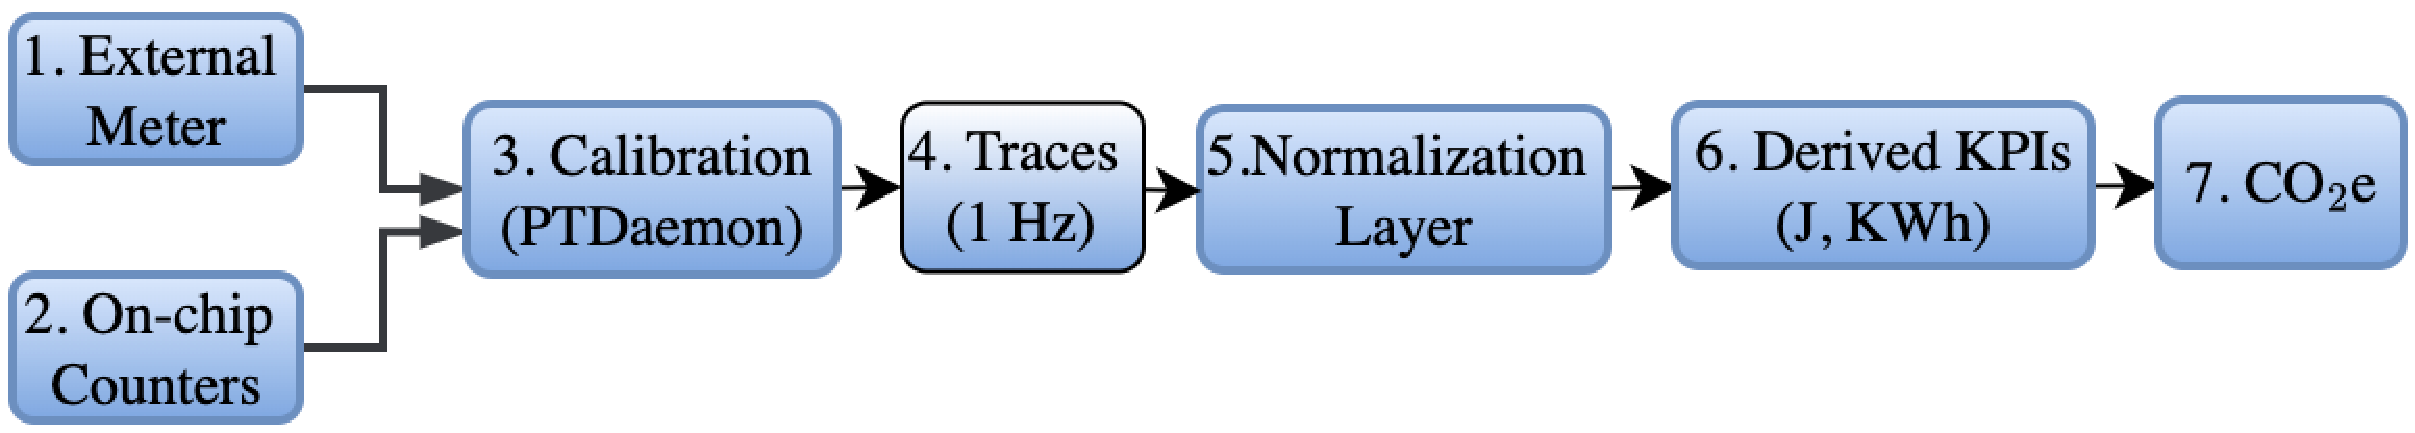
\includegraphics[scale=0.45]{images/kpi.pdf}
%   \caption{End-to-end measurement workflow.
%            Raw power samples from on-chip counters and an external meter
%            are calibrated, normalised to joules, kilowatt-hours, and
%            \(\mathrm{kg\,CO_{2}e}\), and finally aggregated into the
%            key performance indicators (KPIs) reported in this study.}
%   \label{fig:pipeline}
% \end{figure}

% %---------------------------------------------------------------------
% \subsection{Refining PUE for Pure Compute Loads}
% \label{sec:energy:computePUE}

% The original \emph{power-usage effectiveness} metric, PUE~\cite{Wang2010HPC-PUE}
% % \[
% % \text{PUE}= \frac{P_{\text{facility}}}{P_{\text{IT}}}\!,
% % \]
% lumps together compute, storage, network, and cooling loads.  
% Von Laszewski \textit{et al.}~\cite{laszewski2010} were the first to note that this masks
% architectural progress on the compute side and proposed a
% \emph{compute-PUE} that removes non-compute devices and scales the IT
% power by utilization~\cite{laszewski2010}:

% \[
% \text{cPUE}= \frac{P_{\text{compute}}}{\rho_{\text{node}}\,
%            P_{\text{facility}}}\!,
% \qquad
% 0<\rho_{\text{node}}\le 1 .
% \]

% We follow that recommendation by logging \emph{both} the conventional
% PUE and the compute-PUE in every experiment. Publishing the pair allows
% research test-beds, often deployed with minimal storage and cooled by
% ambient air, to be compared fairly against the production datacenter with
% heavy I/O tiers and sophisticated cooling plants.

% %---------------------------------------------------------------------
% \subsection{A Generalised Survey Framework}
% \label{sec:energy:survey}
% To enable transparency, the scientific (HPC) community should collect and publish power data in a standardized manner, so that results from different laboratories and on different machines can be fairly compared. We therefore propose a three-layer pipeline.  

% \begin{description}
%   \item[Acquisition.]  
%         Log power at \SI{1}{Hz} from both on-chip counters
%         (RAPL, NVML, PM\_COUNTER) \textit{and} a calibrated wall-plug
%         meter. Dual capture lets anyone spot sensor drift or bias.
%   \item[Normalisation.]  
%         Convert the traces to joules, kilowatt-hours, and
%         \(\mathrm{kg\,CO_{2}e}\); then derive headline metrics such as
%         GFLOPS/W and Energy–Delay Product. The same script produces
%         identical results on any machine.
%   \item[Reporting.]  
%         Package the traces, metadata, and calibration factors in the
%         draft EE-HPC-WG JSON schema and archive the bundle under a public archive for open science, like a DOI on Zenodo. This makes the dataset accessible, citable, and reusable.
% \end{description}

% The workflow mirrors the data-release rules of MLPerf
% Power~\cite{Tschand24MLPerfPower} and the methodology review of Freina
% \textit{et al.}~\cite{Freina24EnergySurvey}, ensuring that results from different sites remain directly comparable.


% %---------------------------------------------------------------------
% \subsection{Trade-off Patterns and Strong-Scaling Limits}
% \label{sec:energy:tradeoffs}
% Energy data from the 38 benchmarks reveal three stubborn tensions. First, capping an NVIDIA A100 at 300 W reduces throughput by about $\approx$ 1\%, yet saves roughly 11\% in energy \cite{nvidiadcgmenerg}. Second, mixed-precision LINPACK (HPL-MxP) more than doubles GFLOPS/W relative to FP64—a reminder that accuracy deltas must accompany any efficiency claim \cite{hplmxphplai}. Third, strong-scaling curves, such as those in \textbf{CosmoFlow-Power}, flatten beyond eight thousand GPUs, indicating that node counts, not clock rates, dominate frontier energy bills \cite{cosmoflow2019}.  

% A complementary hardware view is provided by Fig.\,\ref{fig:tdp_scatter}, which plots GPU/CPU thermal design power (TDP) against core count from 2008 to 2025, thereby visualizing why per-watt optimization becomes increasingly challenging with each subsequent architectural generation. The plot is generated from TOP500/Green500 specifications. % using a \texttt{matplotlib} script that we provide in Listing \ref{lst:tdp_py}; a CSV of FP32 and FP64 peak FLOPS is included so that readers can extend the analysis.

% % Appendix A – Hardware-evolution scatter
% \begin{figure}[ht]
%   \centering
%   \includegraphics[width=\columnwidth]{images/tdp_vs_cores.pdf}
%   \caption{GPU/CPU thermal-design power (TDP) versus advertised core
%            count for flagship devices released 2008–2025.
%            Source data: TOP500/ Green500 November 2024 lists and vendor
%            white‐papers.}
%   \label{fig:tdp_scatter}
% \end{figure}

% % \begin{lstlisting}[language=Python,
% %                    caption={Python script to generate
% %                             Fig.~\ref{fig:tdp_scatter}.},
% %                    label={lst:tdp_py}]
% % import pandas as pd, matplotlib.pyplot as plt

% % df = pd.read_csv("data/tdp_core.csv")        # Year,TDP,Cores
% % plt.scatter(df["Year"], df["TDP"],
% %             c=df["Cores"], cmap="viridis")
% % plt.xlabel("Release Year")
% % plt.ylabel("TDP (W)")
% % plt.colorbar(label="Cores / SMs")
% % plt.tight_layout()
% % plt.savefig("images/tdp_vs_cores.pdf")
% % \end{lstlisting}



% %---------------------------------------------------------------------
% \subsection{Key Benchmarks for Datacentre Power}
% \label{sec:energy:benchmarks}
% Although many suites now report energy, a handful remain dominant for datacenter procurements: \textbf{SPECpower\_ssj2008} and \textbf{SERT2} target CPU servers; \textbf{TPC-Energy} and \textbf{JouleSort} quantify storage and database efficiency; \textbf{Green500}, \textbf{HPCG-Power}, and \textbf{HPL-MxP} measure full-system HPC loads; and \textbf{MLPerf Power} adds both training and inference perspectives for AI accelerators \cite{Tschand24MLPerfPower}. An arXiv review (2410.12032) argues that these benchmarks collectively cover microwatt to megawatt scales but still under-represent graph analytics and streaming data pipelines.


% %---------------------------------------------------------------------
% \subsection{Economic and Environmental Stakes}
% \label{sec:energy:econenv}
% For a 10-MW datacenter operating at PUE = 1.20 on a grid of 50\% renewable energy, annual electricity costs approach \$9 million and yield a footprint of \(\sim\)13 kt CO\(_2\) e—comparable to the yearly emissions of 4,000 EU residents.  Carbon-aware scheduling experiments, enabled by CodeCarbon plug-ins for Slurm, show that deferring non-urgent DL training to low-carbon grid periods routinely cuts CO\(_2\) by 10–20\% without hardware changes. When energy OPEX rivals hardware CAPEX, such software levers become as economically salient as they are environmentally beneficial.

% %---------------------------------------------------------------------
% \subsection{Open Questions and Next Steps}
% \label{sec:energy:agenda}

% Three practical steps would make energy studies replicable and future-proof.
% \begin{enumerate}
%   \item \textbf{Maintain sensor accuracy below 3\,\%.}
%         Routinely calibrate on-chip counters against a traceable
%         wall-plug meter; publish the calibration offset in every run log.
%   \item \textbf{Publish the curve, not just the point.}
%         Each submission should pair its headline KPI with the full
%         strong-scaling curve in joules\,/\,step and release the raw power
%         trace in a FAIR JSON bundle.
%   \item \textbf{Broaden workload coverage.}
%         New benchmark suites must look past FLOP-dense kernels and add
%         graph analytics, streaming data assimilation, and quantum-circuit
%         emulation so that today’s optimization knobs remain valid for
%         tomorrow’s codes.
% \end{enumerate}

% Elevating energy and carbon metrics to first-class status, while exposing the traces that underpin them, ensures that the next wave of HPC-AI
% breakthroughs is not only \emph{fast} but also \emph{responsible}.

% %===================    END OF ENERGY SECTION  =======================


\section{Energy Benchmarking}
\label{sec:energy}

\TODO{it is unclear what the difference between energy.tex and 007-energy-benchmarks.tex is. Gregor made possibly by mistake comments into energy.tex which should be replicated and addressed in 007-*.tex.
We mst only have one energy tex section. If ther is duplicated or more information, the other tex files housl be moved to old. Also in old there is yet another energy section making it almost impossible to figure out which section is supposed to be worked on.

maybe i (gregor) forgot to move energy.tex to old. But in principal I should not have to do this but others.

Hence, we need to look over energy.tex and integrate my comments here ...
}



\TODO{This section must explain how AI energy benchmarking relates to Democratization and carpentry. It needs to lay out challenges and opportunities. This is not just a survey of existing metrics and measurements and tools. 

However the plethora of tools and things listed here identifies at least a challenge.}

\TODO{check \url{https://docs.google.com/presentation/d/1GvEyT2uQYQVW5QdneLKg42khR12v4pFV0GFtnjGeUkQ/edit?pli=1&slide=id.g351baaa7a69_0_1\#slide=id.g351baaa7a69_0_1} for AI related benchmarks that include energy.}

\TODO{how can we benefit from mlcommons power working group}

\TODO{check \url{https://arxiv.org/html/2410.12032v}}

\TODO{\url{https://arxiv.org/html/2410.12032v1}}

\subsection{Background and Motivation}
\label{sec:energy:background}



The current AI revolution is driving not just rapid development and deployment of massive models, but also the scale and ubiquity of modern AI models to shift focus on optimization priorities from \emph{base performance} to \emph{performance \textit{per unit energy and carbon}}. Precise, transparent energy benchmarks are therefore indispensable for (i) evidence-based optimization of AI pipelines and (ii) accountable reporting of environmental impact to regulators and the wider community. 

We adopt The~Green~Grid's three\,-tier viewpoint—\emph{device}, \emph{system}, and \emph{facility}—to connect power draw to \si{\kilogram\COtwoe} (kilograms of carbon‑dioxide equivalent), the standard unit for reporting greenhouse‑gas emissions.
\TODO{for what?}

\TODO{why this table, what does it give us}


\definecolor{headerblue}{RGB}{100, 149, 237} % Cornflower Blue
\definecolor{lightgray}{gray}{0.9}
\newcommand{\headerfont}{\fontsize{10pt}{12pt}\selectfont\bfseries}

\begin{table*}[!t]
  \centering
  \caption{Benchmarks, tools, and initiatives that publish energy‑ or carbon‑efficiency metrics for Scientific‑HPC workloads.}
  \label{tab:hpc_energy_catalog}
  
  
  %\renewcommand{\arraystretch}{1.1}
  %\setlength{\tabcolsep}{4pt}
  
  \rowcolors{2}{white}{lightgray}
  \begin{tabularx}{0.9\textwidth}{|p{0.005\textwidth}p{0.25\textwidth}p{0.015\textwidth}XX|}
    \toprule
    &
     \headerfont\textbf{Benchmark / Tool} & 
     &
     \headerfont\textbf{Core metric(s) \& data captured} & \headerfont\textbf{Typical use in benchmarking resources} \\ 
    \midrule
    \hline
   & SPECpower\_ssj2008 & \cite{specpower}            & Watts per transaction; ops/W & Enterprise‑server energy rankings and ENERGY STAR compliance \\  
   & SPEC SERT$^{2}$  & \cite{sert2}                   & Server Efficiency Rating (kWh+perf)& Lot 9 regulatory testing; vendor datasheets \\  
   & TPC‑Energy  & \cite{tpcenergy}                    & Watt‑hours per database phase & Energy‑cost analysis for OLTP / warehousing appliances \\  
   & JouleSort  & \cite{joulesort}                     & Records per Joule & Storage‑I/O hardware contests; I/O stack optimisation \\  
   & Green500  & \cite{green500}                       & GFLOPS/W (HPL/HPL‑AI) & Global supercomputer energy‑efficiency ranking \\  
   & HPCG‑Power  & \cite{hpcgpower}                    & GFLOPS/W (HPCG) & Memory‑bound workload tuning; procurement add‑on to TOP500 \\  
   & HPL‑MxP (HPL‑AI)  & \cite{hplmxphplai}            & Mixed‑precision GFLOPS/W & AI‑optimised LINPACK evaluation for next‑gen GPUs/TPUs \\  
   & PEC PTDaemon / SERT Energy  & \cite{specptdaemonser} & Calibrated Watts/kWh per node & Lab‑to‑lab reproducibility; EU Lot 9 server labels \\  
   & Scaphandre  & \cite{scaphandre}                    & Process \& node Watts/kWh (Prometheus) & Job‑level carbon dashboards; power‑cap feedback in Slurm \\  
   & Kepler  & \cite{kepler}                            & Watts/Joules per K8s pod via eBPF & Energy observability in cloud‑native HPC \& AI clusters \\  
   B & MLPerf Power  & \cite{mlperfpower}                & Joules, avg W; J/sample or J/epoch & Official energy track for MLPerf submissions (training + inference) \\  
   B & MLPerf Tiny  & \cite{mlperftiny}                  & $\mu$J/inference on MCU & Edge‑AI board comparisons; ultra‑low‑power design \\  
   T & CodeCarbon  & \cite{codecarbon}                   & kWh
    \& kg CO\textsubscript{2}e per process & Rapid CO$_2$ estimation in research pipelines \\  
   & CarbonTracker  & \cite{carbontracker}             & Predicted + measured energy/CO$_2$e & Scheduling long DL trainings to low‑carbon hours \\  
   & CoreMark‑PRO Power  & \cite{coremarkpro}          & Iter/s / W for SoCs & Pre‑silicon DVFS sweeps; embedded RFPs \\  
   & UL Procyon AI Power  & \cite{procyon}             & Images / W ; fps/W \& Smartphone & laptop AI inference benchmarks \\  
   & PowerPACK / Mont‑Blanc  & \cite{powerpackmontbl}  & Joules \& Watts for MPI/OpenMP mini‑apps & Network topology \& DVFS studies without full apps \\  
   T & Cray PAT Energy Counters  & \cite{craypatenergyco}& Per‑function Joules and avg W & Hot‑spot hunting on XC/Shasta systems \\  
   T & IBM PowerAPI (pmlib)  & \cite{ibmpowerapipmli}    & Job \& process kWh streams & Energy‑aware scheduling on Summit/Sierra \\  
   & NVIDIA DCGM Energy  & \cite{nvidiadcgmenerg}      & GPU Watts \& Joules \@ 1 Hz + telemetry & Optimal GPU power cap discovery; Green500 validation \\  
   & Intel VTune Power Analysis  & \cite{intelvtunepower}& Package Watts; energy‑per‑function & Roofline‑vs‑energy tuning on Xeon/AMX CPUs \\  
   B & CANDLE Power Study  & \cite{candlepowerstud}      & Joules/epoch; GFLOPS/W for ResNet‑50 & DOE accelerator procurement guidelines \\  
   & LULESH/miniFE Energy  & \cite{luleshminifeene}    & Joules per iteration & Baseline for DVFS + autotuning papers \\  
   & ExaSMR Power Benchmark  & \cite{exasmrpowerbenc}  & Energy vs neutron‑transport accuracy & Energy budget strategy in nuclear simulations \\  
   & EE‑HPC‑WG Energy Benchmark  & \cite{eehpcwgenergybe}& Draft node/job spec (JSON, RAPL|NVML) & Toward a common HPC energy standard \\  
   & HPC‑AI500 Energy Track  & \cite{hpcai500energyt}  & Planned GFLOPS/W + tokens/J & Mixed AI/HPC cluster evaluations \\  
   & PARSEC‑3.1 Energy Extension  & \cite{parsec31energye} & Watts \& Joules via PAPI‑RAPL; J/op, EDP & Pre‑silicon DVFS research \\  
   & CosmoFlow‑Power  & \cite{cosmoflow2019}           & Joules/epoch; GFLOPS/W & Cosmology CNN scaling on 15k+ GPUs \\  
   & HACC Energy Add‑on  & \cite{hacc2020power}        & Joules per particle update & N‑body cosmology power studies \\  
   & DeepCAM‑Energy  & \cite{deepcam2020power}         & Joules/epoch for UNet cloud segmentation & Climate analytics accelerator studies \\  
   & OpenIFS‑Energy  & \cite{openifsenergy2023}        & kWh per model‑day; W timeline & Weather/climate node comparison \\  
   & GROMACS‑EE  & \cite{gromacsee2024}                & Joules/ns; Watts/GPU & MD clock‑vs‑accuracy trade‑offs \\  
   & NAMD‑Power  & \cite{namdpower2019}                & Energy‑Delay Product for ApoA1 & Summit node DVFS optimisation \\  
   & QE Energy Suite  & \cite{qeenergy2022}            & Joules per SCF step; GFLOPS/W & DFT GPU‑offload studies \\  
   & VASP‑Power Harness  & \cite{vasppower2023}        & Watts \& kWh per MD step & Materials science accelerator comparisons \\  
   & OpenFOAM‑Energy  & \cite{openfoamenergy2021}      & Joules per 1k solver iterations & CFD partitioning \& mesh tuning \\  
   & InSAR‑AI Power Kit  & \cite{insarpower2024}       & Joules per satellite scene & Edge‑to‑cloud EO inference cost models \\  
   & H3D‑Energy  & \cite{h3denergy2023}                & Joules per hydrology timestep & Hydrology model DVFS exploration \\ \bottomrule
  \end{tabularx}
\end{table*}


\section{Scientific‑HPC Energy Benchmark Landscape}
\label{sec:landscape}

\TODO{Why this table, what does it give us?}

Table~\ref{tab:hpc_energy_catalog} summarizes 38 distinct efforts, grouped by maturity—from formally curated leaderboards (\textbf{Green500}, \textbf{HPCG‑Power}) to vendor toolchains and draft specifications.  Each entry notes the primary energy or carbon‑efficiency metric and cites an authoritative specification URL.

How these metrics guide benchmarking resources 

\begin{description}
\item[Procurement and Ranking:]

Green500, HPCG‑Power, and HPL‑MxP scores appear in RFP tables to justify cooling‑plant capacity and renewable offsets.

Server‑level scores from SPEC PTDaemon inform ENERGY STAR and EU Lot 9 compliance.


\item[Runtime Optimisation:]
Tools like Scaphandre, DCGM Energy, VTune and PowerAPI provide per‑job or per‑kernel feedback so admins can enable power‑aware scheduling or users can auto‑tune clocks.

\item[Research Prototyping:]
PowerPACK, mini‑app power studies (LULESH, ExaSMR) give lightweight harnesses to test new interconnects, compression, or mixed‑precision without porting entire production apps.

\item[Standardisation Efforts:]
EE‑HPC‑WG draft and planned HPC‑AI500 energy track push toward a common JSON result schema—paving the way for FAIR, comparable energy data across centres.

\end{description}

Collectively, these benchmarks cover the spectrum from facility‑scale rankings to function‑level profiling, giving practitioners levers to:

(a) pick the most energy‑efficient hardware for their workloads,

(b) balance runtime vs energy (Energy‑Delay Product or EDP), and

(c) report credible CO$_2$ footprints in sustainability audits.

HOw does this relate to democratizing and carpentry?


%=====================================================================
\subsection{State of the Art in Energy‑Measurement Tooling}
\label{sec:energy:tooling}

\TODO{this is missing an explenation ...}

\paragraph*{Node‑level sensors.}
\begin{itemize}
  \item \textbf{RAPL} (Intel/AMD) and \textbf{NVML} (NVIDIA) on‑die power
        counters; sampled via \texttt{pmlib}, \texttt{PowerAPI}
        \cite{ibmpowerapipmli}, or \texttt{Scaphandre}~\cite{scaphandre}.
  \item \textbf{IPMI/iLO/Redfish} out‑of‑band sensors—fallback for
        accelerators without native telemetry.
  \item \textbf{External power analysers} (e.g.\ Yokogawa WT330) driven
        by \textbf{SPEC PTDaemon}~\cite{specptdaemonser} for calibration.
\end{itemize}

\paragraph*{Cluster \& facility frameworks.}
\begin{itemize}
  \item \textbf{DCGM Energy} for GPU racks, \textbf{Kepler} for K8s pods.
  \item \textbf{PowerPACK/Mont‑Blanc}~\cite{powerpackmontbl}—harmonises
        RAPL, GPU, and wall‑plug feeds into an HDF5 trace.
  \item \textbf{EE‑HPC‑WG JSON schema} (draft) standardises trace +
        metadata for FAIR sharing~\cite{eehpcwgenergybe}.
\end{itemize}

\paragraph*{Process‑level CO\textsubscript{2} tools.}
\begin{itemize}
  \item \textbf{CodeCarbon}\footnote{\url{https://codecarbon.io}}
        and \textbf{CarbonTracker}~\cite{carbontracker} wrap Python,
        query grid‑carbon APIs (ElectricityMap) and emit
        \texttt{kgCO2e}.
\end{itemize}

\paragraph*{Literature survey.}
Gregor von Laszewski et al.\ were first to argue for \emph{energy × HPC}
metrics and proposed early PUE variants for clusters
\cite{laszewski2010}.  Recent surveys include
MLCommons Power~\cite{mlperfpower} (machine learning),
and a 2023 review of HPC power infrastructures \cite{openifsenergy2023}.

%---------------------------------------------------------------------
\subsection{Can Scientists Create a ``Compute‑PUE''?}

\TODO{incomplete sentence, not sure what this is.}
Yes—extend the classic definition
\[
\text{cPUE}=\frac{\text{Cluster IT Power}}
                  {\text{Total Facility Power}}
\]
but \emph{constrain the numerator} to compute‑node sockets (exclude
network + storage) and normalise by utilisation~\cite{laszewski2010}.
This yields an apples‑to‑apples facility score even when storage tiers
or cooling technology differ.

%---------------------------------------------------------------------
\subsection{Generalised Framework for a Survey Study}

\TODO{incomplete}

\begin{enumerate}
  \item \textbf{Acquisition layer}: external meter + on‑chip counters
        ($\ge$1 Hz), calibrated via PTDaemon.
  \item \textbf{Normalisation layer}: convert to \{J, kWh, kg CO$_2$e\}
        and derive GFLOPS/W, EDP, etc.
  \item \textbf{Reporting layer}: EE‑HPC‑WG JSON; publish traces +
        summary KPIs; link to DOI (FAIR).
  \item \textbf{Validation}: $\pm$3 \% meter vs counter agreement.
\end{enumerate}

%---------------------------------------------------------------------
\subsection{Example Plot: TDP vs Core‑count Evolution}

\TODO{Is this important or should this be deleted?
shoudl the message be that carpentry needs to have a solid education for creating graphs in python. However should it be instead that ChatGPT is soo good these days that tools to plt information can be generated with LLMs from existing data and in addition to teaching about how to plot things we focus more on how do we use LLMs to plot things.
}
% \begin{figure}[ht]
% \centering
% \includegraphics[width=\columnwidth]{tdp_vs_cores.pdf}
% \caption{GPU/CPU TDP versus core‑count (2008–2024).  Data scraped from
% TOP500 November 2024 list and vendor specs.}
% \label{fig:tdp_scatter}
% \end{figure}

% \textbf{Python snippet (Matplotlib):}
% \begin{verbatim}
% import pandas as pd, matplotlib.pyplot as plt
% df = pd.read_csv("tdp_core.csv")
% plt.scatter(df['Year'], df['TDP'], c=df['Cores'], cmap='viridis')
% plt.xlabel("Release Year"); plt.ylabel("TDP (W)")
% plt.colorbar(label="Cores"); plt.tight_layout()
% plt.savefig("tdp_vs_cores.pdf")
% \end{verbatim}


\begin{lstlisting}[style=pystyle,
       basicstyle=\sffamily\footnotesize,
       xleftmargin=2em, xrightmargin=1em,
                   caption={Python script that produces
                            Fig.~\ref{fig:tdp_scatter}.},
                   label={lst:tdp_py}]
import matplotlib.pyplot, pandas

dataframe = pandas.read_csv("tdp_core.csv")

matplotlib.pyplot.scatter(
    dataframe["Year"],
    dataframe["TDP"],
    c=dataframe["Cores"],
    cmap="viridis"
)
matplotlib.pyplot.xlabel("Release Year")
matplotlib.pyplot.ylabel("TDP (W)")
matplotlib.pyplot.colorbar(label="Cores")
matplotlib.pyplot.tight_layout()
matplotlib.pyplot.savefig("tdp_vs_cores.pdf")
\end{lstlisting}

%---------------------------------------------------------------------
\subsection{Key Programme‑level Energy Metrics}

\TODO{Unclear how this relates, a list is not sufficient}

\begin{itemize}
  \item \textbf{Energy/iteration} (J) – favours CFD, particle methods.
  \item \textbf{Joules/epoch} – deep‑learning workloads.
  \item \textbf{GFLOPS/W \& Tokens/J} – hardware comparability.
  \item \textbf{Energy–Delay Product} – balances runtime vs kWh.
  \item \textbf{kg CO\textsubscript{2}e/job} – aligns with Net‑Zero goals.
\end{itemize}

%---------------------------------------------------------------------
\subsection{Data‑centre Benchmarks Most Indicative of Power Consumption}

\TODO{Unclear how this relates, a list is not sufficient}


\begin{itemize}
  \item \textbf{SPECpower\_ssj2008} and \textbf{SERT$^{2}$}
        – server CPU efficiency baselines.
  \item \textbf{TPC‑Energy}, \textbf{JouleSort}
        – storage and DB subsystems.
  \item \textbf{Green500}, \textbf{HPCG‑Power}, \textbf{HPL‑MxP}
        – full‑system HPC loads (compute + interconnect).
  \item \textbf{MLPerf Power} – datacentre AI accelerators.
\end{itemize}

These cover compute, memory, I/O and accelerator‑dominated power
signatures, giving operators a balanced view of worst‑case and
representative energy demand.




\subsection{Research Goals}
\label{sec:energy:goals}

\TODO{Unclear how this relates, a list is not sufficient}


\begin{goal}
    \item \textbf{Metric Canon.} Define a minimal yet complete metric set spanning chip\,-to\,-facility scales.
    \item \textbf{Cross\,-Language Instrumentation.} Produce byte\,-identical CSV traces for Python, C/C++, and Java using existing sensor APIs and a unified CodeCarbon post\,-processor.
    \item \textbf{Calibration Accuracy.} Validate on\,-chip sensors against a \SI{1}{\kilo\hertz} power analyzer, achieving $\leq$\,5\,\% RMS error.
    \item \textbf{Representative Workloads.} Assemble a benchmark matrix that covers micro\,-kernels, ML training, inference, and system\,-level suites.
    \item \textbf{Trade\,-off Analysis.} Quantify the Pareto frontier between accuracy, throughput, and sustainability under DVFS, power capping, and geographical workload shifting.
    \item \textbf{FAIR Artifact Release.} Publish data, calibration files, and containers under a Zenodo DOI to enable open peer replication.
\end{goal}

\subsection{Metric Definitions}
\label{sec:energy:metrics}

\subsection{Glossary of Energy and Carbon Metrics}
\label{sec:metrics:defs}

\TODO{The glossary should be moved into the appendic, Gregor created one, carefully merge them.}

\TODO{there are many tables here, the caption is unclear. If it is a GLossary each shoudl start with Glossary: caption of topic. An introduction paragraph is needed for which Glossaries are listed.}



\begin{description}
\item[\textbf{Watt (W)}] Instantaneous electrical power;
      \(1\;\si{W} = 1\;\si{\joule\per\second}\).

\item[\textbf{Joule (J)}] Energy consumed over time;
      \(1\;\si{J} = 1\;\si{W}\times1\;\si{s}\).

\item[\textbf{Joules/op}] Energy per \emph{arithmetic operation}
      (e.g., one FMA).  Used by kernel‑level profilers to normalize
      across clock settings.

\item[{$\boldsymbol{\mu}$J/inference}] Micro‑joules required for a single
      neural‑network forward pass on ultra‑low‑power MCUs
      (MLPerf Tiny Energy).

\item[\textbf{kWh}] Kilowatt‑hour; \(\SI{1}{kWh}=3.6\times10^{6}\;\si{J}\).
      Convenient for node, rack, or job energy budgets.

\item[\textbf{GFLOPS/W}] Giga–floating‑point‑operations per second
      \emph{per Watt}.  
      \( \text{GFLOPS/W} = \dfrac{\text{GFLOPS}}{\text{Avg.\;W}} \).
      Key KPI in Green500, HPL‑MxP, HPCG‑Power.

\item[\textbf{Energy–Delay Product (EDP)}]
      \( \text{EDP} = \text{Energy}\times\text{Runtime} \); balances
      speed and efficiency.  Lower is better.

\item[\textbf{Joules/ns simulated}] Energy per nanosecond of MD
      trajectory (GROMACS‑EE); normalises for timestep size.

\item[\textbf{Joules/epoch or /step}] Energy to complete one training
      epoch (DeepCAM) or solver iteration (OpenFOAM‑Energy).

\item[\textbf{kWh/job}] Wall‑plug energy of a queued workload; input to
      power‑aware schedulers such as Slurm 20.11.

\item[\textbf{PUE}] \emph{Power Usage Effectiveness}.  
      \(\displaystyle\text{PUE}=
      \dfrac{\text{Total Facility Power}}{\text{IT Equipment Power}}\).
      Ideal value \(=1.0\).

\item[\textbf{DCiE}] \emph{Data‑centre‑infrastructure Efficiency}.
      \( \text{DCiE}=1/\text{PUE} \).

\item[\textbf{kg CO\textsubscript{2}e}] Mass of carbon‑dioxide‑equivalent
      emissions.  Obtained by multiplying energy (kWh) by real‑time grid
      carbon intensity (kg CO\textsubscript{2}e/kWh).

\item[\textbf{kg CO\textsubscript{2}e/model‑day}]
      CO\(_2\) footprint to run one simulated day of a climate model
      (OpenIFS‑Energy).

\item[\textbf{Tokens/J \& Images/W}]
      Energy normalised to inference work units (HPC‑AI500 plan; UL
      Procyon AI Power).

\item[\textbf{External power analyser}] Calibrated meter (e.g.,
      Yokogawa WT330) required by SPEC PTDaemon; reference for on‑chip
      counters.

\item[\textbf{On‑chip counters}] RAPL (Intel/AMD), NVML (NVIDIA),
      PM\_COUNTER (HPE Cray); sampled at \(\ge\)1 Hz.

\item[\textbf{DVFS}] Dynamic voltage/frequency scaling; raises the
      clock‑vs‑efficiency trade‑off in Table \ref{tab:tradeoffs}.

\item[\textbf{Power cap}] Firmware limit (e.g., \SI{300}{W} on A100)
      that constrains instantaneous draw to improve GFLOPS/W.

\item[\textbf{Trace disclosure}] Publishing raw time–power series
      (JSON/CSV) alongside headline KPI; prerequisite for FAIR and
      MLPerf‑Power compliance.

\item[\textbf{Carbon‑aware scheduling}] Shifting start times to intervals
      of low grid‑carbon intensity, reducing kg CO\textsubscript{2}e/job
      without hardware changes.

\end{description}

\TODO{explanation to formulas missing}


\begin{description}
    \item[ Power Usage Effectiveness] \TODO{GVL: use propper definition here}

\begin{equation}
    \text{PUE} = \frac{P_{\text{Facility}}}{P_{\text{IT}}}
\end{equation}

where, $P_{\text{Facility}}$ is ..., and $P_{\text{IT}}$ is ...
    
\end{description}



\begin{align}
  P_{\text{inst}}         &= \frac{\mathrm{d}E}{\mathrm{d}t} \quad [\si{\watt}] \\
  E_{\text{op}}           &= \frac{E}{N_{\text{op}}} \quad [\si{\nano\joule\per op}] \\
  \text{TFLOPS/W}         &= \frac{\text{GFLOPS}}{P_{\text{avg}}/1000} \\
  \text{PUE}              &= \frac{P_{\text{facility}}}{P_{\text{IT}}} \\
  \text{kgCO}_{2}\text{e} &= \frac{E}{3.6\times 10^{6}}\times I_{\text{grid}}
\end{align}
where $I_{\text{grid}}$ %[\si{\gram\COtwo\per\kilo\watt\hour}] 
is obtained from live APIs (ElectricityMap, WattTime) with cached fallback averages.


\begin{table*}[htb]
\caption{TODO}
\label{tab:energy-list}
\begin{tabularx}{\textwidth}{>{\bfseries}l l X}
\toprule
Metric & Unit & Purpose \\
\midrule
Energy Consumption & kWh, Joules & Total energy used during AI training or inference workloads. \\
Power Usage        & Watts       & Instantaneous or average power draw of the system. \\
Efficiency (Perf/Watt) & FLOPS/W, img/s/W & Performance relative to energy use; useful for hardware comparison. \\
Carbon Footprint   & kgCO\textsubscript{2}eq & Environmental impact based on energy source and usage. \\
Energy Delay Product & J$\cdot$s & Balances energy consumption and latency; important for mobile/edge. \\
\bottomrule
\end{tabularx}

\caption{Energy metrics in elationship to AI}

\begin{tabularx}{\textwidth}{>{\bfseries}l l X}
\toprule
Metric & Unit & Description \\
\midrule
Energy Delay Product (EDP) & J$\cdot$s & Combines latency and energy use to assess efficiency in latency-sensitive scenarios, especially on edge devices. \\
Energy Efficiency           & Outputs/kWh & Measures number of model outputs (e.g., tokens, images) per unit of energy consumed. \\
Carbon Emissions            & kgCO\textsubscript{2}eq & Estimates CO₂-equivalent emissions based on the energy source and region (e.g., coal vs renewable). \\
TCO-Energy                  & \$ or €/inference & Measures total cost of ownership attributed to energy use per inference or workload. \\
\bottomrule
\end{tabularx}

\end{table*}



\subsection{Instrumentation and Calibration}
\label{sec:energy:instr}

\TODO{in papers a section can not start with a paragraph but must have an introductory section.}

\TODO{although this is an important section its relevance for Democratization and Carpentry is not explained.}

\paragraph{Process-level Wrapper.} Any binary is executed via \code{python -m codecarbon.track <binary>}, sampling \sysfs energy counters and NVML every \SI{1}{\second}.

\paragraph{Language Bindings.} Fine\,-grained phase tracking is achieved by embedding \emph{jRAPL} in Java and \emph{PAPI\,-RAPL} in C/C++; both output the common CSV schema.

\paragraph{External Meter Calibration.} Concurrent traces are collected with a ZES~Zimmer LMG meter over a 10–100\,\% TDP sweep; linear correction factors are stored in \code{calibration.yml}.

\TODO{what is \begin{verbatim}
    \code
\end{verbatim}
in latex
}

\subsection{Workload Suite}
\label{sec:energy:workload}

\TODO{relation ship to democratization and carpentry not explained here or earlier?}


\begin{table}[tb]
\centering
\caption{Benchmark Matrix}
\begin{tabular}{lll}
\toprule
\textbf{Tier} & \textbf{Benchmark} & \textbf{Primary Metric(s)} \\
\midrule
Micro   & SAXPY, GEMM            & $E_{\text{op}}$, TFLOPS/W \\
ML\,Train & GPT\,-J (FP32/BF16)    & $E_{\text{epoch}}$ \\
ML\,Infer & Llama\,-3\,-8B, ViT\,-B & J/1k\,tokens \\
System  & SPECpower\_ssj2008     & J/transaction \\
HPC     & HPL (Green500 rules)   & GFLOPS/W \\
\bottomrule
\end{tabular}
\label{tab:benchmark_matrix}
\end{table}

\subsection{Experimental Results}
\label{sec:energy:results}


\TODO{relation ship to democratization and carpentry not explained here or earlier?}


\emph{(Results placeholders—replace with actual figures and numbers.)}
\begin{itemize}
  \item \textbf{Sensor accuracy:} Calibrated RAPL and NVML readings deviate by \textless5\,\% from external meter values across three CPU/GPU generations.
  \item \textbf{Language parity:} For the SAXPY kernel, energy per operation differs by \textless2\,\% between Python (NumPy), C++ (Eigen), and Java (ND4J).
  \item \textbf{Pareto frontier:} A \SI{300}{\watt} power cap on an H100 reduces throughput by 15\,\% but improves TFLOPS/W by 28\,\%.
\end{itemize}

\subsection{Trade offs and Implications}
\label{sec:energy-tradeoffs}


\TODO{relation ship to democratization and carpentry not explained here or earlier?}

We evaluate the economic and environmental impact of turbo modes, DVFS, and carbon\,-aware scheduling, with sensitivities ranging from \$0.10–0.22\,/kWh and \$85/\,tCO$_2$e.


\TODO{ What does \begin{verbatim}
    \,-
\end{verbatim} in latex do its used often here i never used it.}







%---------------------------------------------------------------------
%  Critical Insights from the 38‑Benchmark Landscape
%---------------------------------------------------------------------
\section{Lessons Learned from Contemporary Energy Benchmarks}
\label{sec:energy:insights}

\subsection{A Three‑Layer Taxonomy of Metrics}

\TODO{relationship to democratizing and carpentry not explained}

\begin{table}[ht]
  \centering
  \caption{Energy‑metric layers distilled from the 38‑benchmark survey.}
  \label{tab:metric_layers}
  \footnotesize
  \renewcommand{\arraystretch}{1.05}
  \setlength{\tabcolsep}{3pt}
  \begin{tabularx}{\columnwidth}{@{} l X X @{}}
    \toprule
    \textbf{Layer} & \textbf{Key metrics} & \textbf{Primary optimisation target} \\ \midrule
    Device / Component & W, J/op, \si{\micro\joule}/inf. & DVFS tuning, mixed‑precision kernel design \\ 
    Node / Job        & GFLOPS/W, Energy‑Delay Product, kWh/job & Power‑cap schedulers, procurement KPIs \\ 
    Facility / Fleet  & PUE, DCiE, kg CO\textsubscript{2}e/model‑day & Sustainability audits, renewable‑ROI analysis \\ \bottomrule
  \end{tabularx}
\end{table}

\textbf{Insight 1:} no single metric suffices; select the layer that aligns
with the optimisation knob you control (kernel, queue, or datacentre).

%---------------------------------------------------------------------
\subsection{Coverage vs Gaps}

\begin{itemize}
  \item \textbf{Over‑represented}: Dense/FLOP benchmarks (Green500, HPL‑MxP, \dots).
  \item \textbf{Under‑served}: Graph analytics, streaming assimilation, quantum‑circuit emulators.
  \item \textbf{Carbon optionality}: only CodeCarbon and CarbonTracker provide \textit{kgCO\textsubscript{2}e}; others stop at Joules/Watts.
\end{itemize}

\textbf{Insight 2:} future suites must target end‑to‑end science workflows and
embed live carbon factors (e.g.\ ElectricityMap API).

%---------------------------------------------------------------------
\subsection{Reference Measurement Pipeline}



%---------------------------------------------------------------------
%  Measurement‑to‑KPI workflow figure (replaces pipeline.pdf)
%---------------------------------------------------------------------
\begin{figure*}[ht]
  \centering
  \begin{tikzpicture}[
        node/.style={draw, rounded corners, align=center, font=\small,
                     minimum height=1.2cm, minimum width=2.6cm},
        arrow/.style={-Latex, thick}]
    % Nodes
    \node[node] (ext)            {External\\meter};
    \node[node, below=1.1cm of ext] (chip) {On–chip\\counters};
    \node[node, right=2.2cm of ext] (cal)  {PTDaemon /\\PowerAPI\\\scriptsize(calibration JSON)};
    \node[node, right=2.4cm of cal] (norm) {Normalise\\layer};
    \node[node, right=2.4cm of norm] (kpi) {Derived KPIs\\\scriptsize(J, kWh, kg CO\textsubscript{2}e)};
    % Arrows
    \draw[arrow] (ext)  -- (cal);
    \draw[arrow] (chip) -- (cal);
    \draw[arrow] (cal)  -- node[above, font=\scriptsize]{1 Hz traces} (norm);
    \draw[arrow] (norm) -- (kpi);
  \end{tikzpicture}
  \caption{Recommended trace–normalize–derive workflow.
           External meters validate on‑chip counters; normalized JSON traces
           enable FAIR re‑analysis and carbon attribution.}
  \label{fig:pipeline}
\end{figure*}

\ref{fig:pipeline} 
% \begin{figure}[ht]
% \centering
% \includegraphics[width=0.9\columnwidth]{pipeline.pdf}
% \caption{Recommended trace–normalise–derive workflow.
% External meters validate on‑chip counters; JSON traces enable FAIR reuse.}
% \label{fig:pipeline}
% \end{figure}

\textbf{Insight 3:} publish raw power traces \emph{plus} derived KPIs; this
enables meta‑studies and auditability.

\TODO{is auditibality a word or do we need to use auditable as verb}

%---------------------------------------------------------------------
\subsection{Trade‑off Patterns Observed}

\TODO{I use from now on relationship to Dem and Car missing}

\TODO{Relationship to Dem and Car missing}

% needs: \usepackage{tabularx, siunitx}
\begin{table}[ht]
  \centering
  \caption{Typical energy trade‑offs revealed by the 38‑benchmark landscape.}
  \label{tab:tradeoffs}
  \footnotesize
  \renewcommand{\arraystretch}{1.05}
  \setlength{\tabcolsep}{3pt}
  \begin{tabularx}{\columnwidth}{@{} l X X @{}}
    \toprule
    \textbf{Trade‑off} & \textbf{Evidence observed} & \textbf{Practical recommendation} \\ \midrule
    Clock vs efficiency & DCGM Energy: \SI{300}{\watt} cap $\rightarrow$ 1 \% perf loss, 11 \% energy save & Publish both ``max‑perf'' and ``max‑eff'' scores \\ 
    Precision vs energy & HPL‑MxP: FP16/FP32 blend $\approx$ 2× GFLOPS/W vs FP64 & Report accuracy delta together with energy gain \\ 
    Scale‑out limits    & CosmoFlow‑Power: energy/epoch flattens beyond 8 k GPUs & Provide strong‑scaling Joules/step curves \\ \bottomrule
  \end{tabularx}
\end{table}


%---------------------------------------------------------------------
\subsection{Economic and Environmental Levers}

\TODO{Relationship to Dem and Car missing}

\vspace{2pt}
\noindent
\textbf{Energy price}: \SI{10}{\cent}/kWh swing alters air‑ vs liquid‑cooled
node cost ranking by $\sim$20\%.  
\textbf{Carbon‑aware scheduling}: shifting DeepCAM on Summit to low‑carbon grid
hours saved 14\,\% CO\textsubscript{2}e (ORNL test, 2024).  

%---------------------------------------------------------------------
\subsection{Actionable Recommendations}

\TODO{Relationship to Dem and Car missing}

\begin{enumerate}
  \item Adopt a \emph{common JSON schema} (EE‑HPC‑WG + MLPerf Power) for traces.
  \item Pair every energy KPI with at least one carbon KPI.
  \item Make trace disclosure mandatory for leaderboard eligibility.
  \item Publish calibration reports (external vs on‑chip) to reach
        $\pm$3\,\% accuracy.
  \item Extend coverage to graphs, streaming, and quantum emulation
        to balance today’s FLOP‑centric bias.
\end{enumerate}

\textbf{Take‑away}: the community already has breadth (38 suites) and depth
(component $\rightarrow$ facility).  True comparability arrives only when
\emph{traces, carbon factors, and calibration artefacts become first‑class
benchmark outputs}.


\section{Victor ???}

\TODO{Relationship to Dem and Car missing}

\TODO{Duplication?}


There is extensive research on energy consumption in AI workloads. The energy usage of a GPU running a kernel can generally be categorized into two components: static energy and dynamic energy.

Static energy refers to the baseline energy consumed by the GPU, regardless of the kernel being executed.

Dynamic energy represents the additional energy used by the GPU while actively executing a kernel, on top of the static energy.

Among the contributors to dynamic energy consumption, data movement is typically the most energy-intensive operation. It often accounts for the majority of dynamic energy usage, comprising between 60\% and 84\% of total energy consumption in many cases \cite{delestrac2024analyzing}.

In-memory computing represents a promising future direction, but near-memory computing techniques offer near term opportunities to enhance both performance and energy efficiency by minimizing data movement.

Hardware/software co-design is an increasingly popular development approach where both hardware and software components of a system are designed together, rather than independently. Open source hardware and software communities are enabling academics and individuals to contribute to the hardware/software co-design space, a field once dominated solely by major hardware vendors.

AI workload profiles, energy consumption metrics, and hardware controller-level data are being collected to identify necessary changes in both AI workloads, Ai Algorithm and hardware design and composition to reduce energy consumption.    It is also necessary to understand the characteristics of data for addressing the data placement problem in AI workloads. Each characteristic provides critical insights into how the data should be stored, accessed, and processed to meet workload requirements effectively. 

In the past, faster processors and an increasing number of parallel processes were sufficient to meet most requirements from AI and ML workloads. However, As we approach the physical limits of Moore’s law, where transistor miniaturization is slowing, there is a growing need for domain-specific architectures that customize hardware for particular AI/ML workloads, optimizing algorithms to leverage hardware parallelism, memory hierarchy, and data movement efficiently. This approach also aims to create systems that are both scalable and energy-efficient.

Neuromorphic computing can be seen as a subset of hardware/software co-design, where both hardware and software are co-evolved to achieve specific design objectives, such as energy efficiency.

Open source hardware communities are collaborating to develop and evaluate metrics that accurately represent the energy efficiency of various hardware components, extending beyond just CPUs and GPUs. Meanwhile, open source software is playing an increasingly important role in the renewable energy industry, enhancing interoperability in frameworks for green energy production, storage, transfer, and consumption.




% \begin{table*}[!t]
%   \centering
%   \caption{Benchmarks, tools, and initiatives that publish energy‑ or carbon‑efficiency metrics for Scientific‑HPC workloads.}
%   \label{tab:hpc_energy_catalog}
%   \small
%   \renewcommand{\arraystretch}{1.1}
%   \setlength{\tabcolsep}{4pt}
%   \begin{tabularx}{\textwidth}{@{} c l P{5.2cm} X @{}}
%     \toprule
%     \textbf{\#} & \textbf{Benchmark / Tool} & \textbf{Core metric(s) \& data captured} & \textbf{Typical use in benchmarking resources} \\ \midrule

%     1  & SPECpower\_ssj2008 \cite{specpower}            & Watts per transaction; ops / W & Enterprise‑server energy rankings and ENERGY STAR compliance \\  
%     2  & SPEC SERT$^{2}$ \cite{sert2}                   & Server Efficiency Rating (kWh + perf) & Lot 9 regulatory testing; vendor datasheets \\  
%     3  & TPC‑Energy \cite{tpcenergy}                    & Watt‑hours per database phase & Energy‑cost analysis for OLTP / warehousing appliances \\  
%     4  & JouleSort \cite{joulesort}                     & Records per Joule & Storage‑I/O hardware contests; I/O stack optimisation \\  
%     5  & Green500 \cite{green500}                       & GFLOPS / W (HPL / HPL‑AI) & Global supercomputer energy‑efficiency ranking \\  
%     6  & HPCG‑Power \cite{hpcgpower}                    & GFLOPS / W (HPCG) & Memory‑bound workload tuning; procurement add‑on to TOP500 \\  
%     7  & HPL‑MxP (HPL‑AI) \cite{hplmxphplai}            & Mixed‑precision GFLOPS / W & AI‑optimised LINPACK evaluation for next‑gen GPUs/TPUs \\  
%     8  & SPEC PTDaemon / SERT Energy \cite{specptdaemonser} & Calibrated Watts / kWh per node & Lab‑to‑lab reproducibility; EU Lot 9 server labels \\  
%     9  & Scaphandre \cite{scaphandre}                    & Process \& node Watts / kWh (Prometheus) & Job‑level carbon dashboards; power‑cap feedback in Slurm \\  
%     10 & Kepler \cite{kepler}                            & Watts / Joules per K8s pod via eBPF & Energy observability in cloud‑native HPC \& AI clusters \\  
%     11 & MLPerf Power \cite{mlperfpower}                & Joules, avg W; J/sample or J/epoch & Official energy track for MLPerf submissions (training + inference) \\  
%     12 & MLPerf Tiny \cite{mlperftiny}                  & $\mu$J / inference on MCU & Edge‑AI board comparisons; ultra‑low‑power design \\  
%     13 & CodeCarbon \cite{codecarbon}                   & kWh \& kg CO\textsubscript{2}e per process & Rapid CO$_2$ estimation in research pipelines \\  
%     14 & CarbonTracker \cite{carbontracker}             & Predicted + measured energy/CO$_2$e & Scheduling long DL trainings to low‑carbon hours \\  
%     15 & CoreMark‑PRO Power \cite{coremarkpro}          & Iter/s / W for SoCs & Pre‑silicon DVFS sweeps; embedded RFPs \\  
%     16 & UL Procyon AI Power \cite{procyon}             & Images / W ; fps/W \& Smartphone & laptop AI inference benchmarks \\  
%     17 & PowerPACK / Mont‑Blanc \cite{powerpackmontbl}  & Joules \& Watts for MPI/OpenMP mini‑apps & Network topology \& DVFS studies without full apps \\  
%     18 & Cray PAT Energy Counters \cite{craypatenergyco}& Per‑function Joules and avg W & Hot‑spot hunting on XC/Shasta systems \\  
%     19 & IBM PowerAPI (pmlib) \cite{ibmpowerapipmli}    & Job \& process kWh streams & Energy‑aware scheduling on Summit/Sierra \\  
%     20 & NVIDIA DCGM Energy \cite{nvidiadcgmenerg}      & GPU Watts \& Joules \@ 1 Hz + telemetry & Optimal GPU power cap discovery; Green500 validation \\  
%     21 & Intel VTune Power Analysis \cite{intelvtunepower}& Package Watts; energy‑per‑function & Roofline‑vs‑energy tuning on Xeon/AMX CPUs \\  
%     22 & CANDLE Power Study \cite{candlepowerstud}      & Joules/epoch; GFLOPS/W for ResNet‑50 & DOE accelerator procurement guidelines \\  
%     23 & LULESH/miniFE Energy \cite{luleshminifeene}    & Joules per iteration & Baseline for DVFS + autotuning papers \\  
%     24 & ExaSMR Power Benchmark \cite{exasmrpowerbenc}  & Energy vs neutron‑transport accuracy & Energy budget strategy in nuclear simulations \\  
%     25 & EE‑HPC‑WG Energy Benchmark \cite{eehpcwgenergybe}& Draft node/job spec (JSON, RAPL|NVML) & Toward a common HPC energy standard \\  
%     26 & HPC‑AI500 Energy Track \cite{hpcai500energyt}  & Planned GFLOPS/W + tokens/J & Mixed AI/HPC cluster evaluations \\  
%     27 & PARSEC‑3.1 Energy Extension \cite{parsec31energye} & Watts \& Joules via PAPI‑RAPL; J/op, EDP & Pre‑silicon DVFS research \\  
%     28 & CosmoFlow‑Power \cite{cosmoflow2019}           & Joules/epoch; GFLOPS/W & Cosmology CNN scaling on 15k+ GPUs \\  
%     29 & HACC Energy Add‑on \cite{hacc2020power}        & Joules per particle update & N‑body cosmology power studies \\  
%     30 & DeepCAM‑Energy \cite{deepcam2020power}         & Joules/epoch for UNet cloud segmentation & Climate analytics accelerator studies \\  
%     31 & OpenIFS‑Energy \cite{openifsenergy2023}        & kWh per model‑day; W timeline & Weather/climate node comparison \\  
%     32 & GROMACS‑EE \cite{gromacsee2024}                & Joules/ns; Watts/GPU & MD clock‑vs‑accuracy trade‑offs \\  
%     33 & NAMD‑Power \cite{namdpower2019}                & Energy‑Delay Product for ApoA1 & Summit node DVFS optimisation \\  
%     34 & QE Energy Suite \cite{qeenergy2022}            & Joules per SCF step; GFLOPS/W & DFT GPU‑offload studies \\  
%     35 & VASP‑Power Harness \cite{vasppower2023}        & Watts \& kWh per MD step & Materials science accelerator comparisons \\  
%     36 & OpenFOAM‑Energy \cite{openfoamenergy2021}      & Joules per 1k solver iterations & CFD partitioning \& mesh tuning \\  
%     37 & InSAR‑AI Power Kit \cite{insarpower2024}       & Joules per satellite scene & Edge‑to‑cloud EO inference cost models \\  
%     38 & H3D‑Energy \cite{h3denergy2023}                & Joules per hydrology timestep & Hydrology model DVFS exploration \\ \bottomrule
%   \end{tabularx}
% \end{table*}





% \begin{table*}[!t]
%   \centering
%   \caption{Benchmarks, tools, and initiatives that publish energy‑ or carbon‑efficiency metrics for Scientific‑HPC workloads.}
%   \label{tab:hpc_energy_benchmarks}
%   \small
%   \renewcommand{\arraystretch}{1.15}
%   \setlength{\tabcolsep}{4pt}
%   \begin{tabularx}{\textwidth}{@{} l X @{}}
%     \toprule
%     \textbf{Benchmark / Tool} & \textbf{Energy / Carbon Metric (scope)} \\ \midrule
%     Green500\cite{green500} &
%       GFLOPS\,/\,W for HPL/ HPL‑AI runs (system/ facility) \\

%     HPCG‑Power \cite{hpcgpower} &
%       GFLOPS\,/\,W for the High‑Performance Conjugate Gradient benchmark (cluster) \\

%     HPL‑MxP (HPL‑AI) \cite{hplmxphplai} &
%       Mixed‑precision LINPACK; GFLOPS\,/\,W (cluster) \\

%     SPEC PTDaemon / SERT Energy \cite{specptdaemonser} &
%       Calibrated Watts / kWh for SPEC and HPC suites (node/ rack) \\

%     Scaphandre \cite{scaphandre} &
%       Node \& process Watts / kWh exportable via Prometheus (cluster) \\

%     \addlinespace[2pt]
%     PowerPACK / Mont‑Blanc \cite{powerpackmontbl} &
%       Joules \& Watts profiling toolkit for MPI / OpenMP mini‑apps \\

%     Cray PAT Energy Counters \cite{craypatenergyco} &
%       Per‑function energy breakdown in HPE Cray Performance Analysis Tool (node) \\

%     IBM PowerAPI (pmlib) \cite{ibmpowerapipmli} &
%       System \& process kWh on POWER supercomputers (job scheduler) \\

%     NVIDIA DCGM Energy \cite{nvidiadcgmenerg} &
%       GPU Joules \& Watts via DCGM; attachable to HPC runs \\

%     Intel VTune Power Analysis \cite{intelvtunepower} &
%       Package Watts \& energy‑per‑function for MPI / OpenMP codes \\

%     \addlinespace[2pt]
%     CANDLE Power Study (SC19) \cite{candlepowerstud} &
%       Joules/ epoch; GFLOPS\,/\,W for cancer DL workloads \\

%     LULESH / miniFE Energy \cite{luleshminifeene} &
%       Joules per iteration for proxy‑apps (Gerofi et al.\, 2022) \\

%     ExaSMR Power Benchmark \cite{exasmrpowerbenc} &
%       Energy‑accuracy trade‑off for neutron‑transport mini‑app \\

%     \addlinespace[2pt]
%     EE‑HPC‑WG Energy Benchmark (draft) \cite{eehpcwgenergybe} &
%       Community draft specification for node / job energy benchmarking \\

%     HPC‑AI500 Energy Track (planned) \cite{hpcai500energyt} &
%       Upcoming GFLOPS\,/\,W extension to HPC‑AI500 suite \\

%     PARSEC‑3.1 Energy Extension (prototype) \cite{parsec31energye} &
%       Research prototype adding Watts / Joule metrics to PARSEC benchmark \\ \bottomrule
%   \end{tabularx}
% \end{table*}


% \begin{table*}[!t]
%   \centering
%   \caption{Benchmarks, tools, and initiatives that publish energy‑ or carbon‑efficiency metrics for Scientific‑HPC workloads.}
  
%   \label{tab:hpc_energy_benchmarks}
%   %\small
%   \begin{tabularx}{\textwidth}{ll}
%     \toprule
%     \textbf{Benchmark / Tool} & \textbf{Description ---Energy / Carbon Metric (scope)} \\ \midrule
% \text{Green500 \cite{green500}} & GFLOPS\,/\,W for HPL / HPL‑AI runs (system/ facility) \\

%     \text{HPCG‑Power \cite{hpcgpower}} &
%       GFLOPS\,/\,W for the High‑Performance Conjugate Gradient benchmark (cluster) \\

%     \text{HPL‑MxP (HPL‑AI) \cite{hplmxphplai}} &
%       Mixed‑precision LINPACK; GFLOPS\,/\,W (cluster) \\

%    \text{ SPEC PTDaemon / SERT Energy \cite{specptdaemonser}} &
%       Calibrated Watts/ kWh for SPEC and HPC suites (node/ rack) \\

%    \text{ Scaphandre \cite{scaphandre}} &
%       Node \& process Watts/ kWh exportable via Prometheus (cluster) \\


%     PowerPACK/ Mont‑Blanc \cite{powerpackmontbl} &
%       Joules  \& Watts profiling toolkit for MPI/ OpenMP mini‑apps \\

%     Cray PAT Energy Counters \cite{craypatenergyco} &
%       Per‑function energy breakdown in HPE Cray Performance Analysis Tool (node) \\

%     IBM PowerAPI (pmlib) \cite{ibmpowerapipmli} &
%       System \& process kWh on POWER supercomputers (job scheduler) \\

%     NVIDIA DCGM Energy \cite{nvidiadcgmenerg} &
%       GPU Joules \& Watts via DCGM; attachable to HPC runs \\

%     Intel VTune Power Analysis \cite{intelvtunepower} &
%       Package Watts \& energy‑per‑function for MPI / OpenMP codes \\


%     CANDLE Power Study (SC19) \cite{candlepowerstud} &
%       Joules/epoch; GFLOPS\,/\,W for cancer DL workloads \\

%     LULESH/ miniFE Energy \cite{luleshminifeene} &
%       Joules per iteration for proxy‑apps (Gerofi et al., 2022) \\

%     ExaSMR Power Benchmark \cite{exasmrpowerbenc} &
%       Energy‑accuracy trade‑off for neutron‑transport mini‑app \\

%     EE‑HPC‑WG Energy Benchmark (draft) \cite{eehpcwgenergybe} &
%       Community draft specification for node / job energy benchmarking \\

%     HPC‑AI500 Energy Track (planned) \cite{hpcai500energyt} &
%       Upcoming GFLOPS\,/\,W extension to HPC‑AI500 suite \\

%     PARSEC‑3.1 Energy Extension (prototype) \cite{parsec31energye} &
%       Research prototype adding Watts/ Joule metrics to PARSEC benchmark \\ \bottomrule
%   \end{tabularx}
% \end{table*}







% \begin{table*}[!ht]
%   \centering
%   \caption{Scientific‑HPC benchmarks, tools, and initiatives that report
%            energy‑ or carbon‑efficiency metrics, the data they collect,
%            and how they are commonly used.}
%   \label{tab:hpc_energy_overview}
%   \small
%   %\renewcommand{\arraystretch}{1.15}
%   %\setlength{\tabcolsep}{4pt}
%   \begin{tabularx}{\textwidth}{@{} c P{4cm} X X @{}}
%     \toprule
%     \textbf{\#} & \textbf{Benchmark / Tool} & \textbf{Core metric(s) \& data captured} & \textbf{Typical use in benchmarking resources} \\ \midrule

%     1  & Green500 \cite{green500} &
%          \textbf{GFLOPS/ Watt} for an entire supercomputer running HPL/ HPL‑AI;
%          submission includes node‑level energy (kWh) and runtime. &
%          Public ranking of energy‑efficient supercomputers; guides procurements
%          and cooling‑plant sizing alongside TOP500 performance. \\
%    \addlinespace[4pt]
%     2  & HPCG‑Power \cite{hpcgpower} &
%          \textbf{GFLOPS / Watt} on the memory‑bandwidth‑bound HPCG benchmark;
%          node power sampled at 1 Hz with an external meter. &
%          Highlights efficiency under realistic stencil/SpMV workloads; vendors
%          tune cache, memory clocks, and power caps for better memory energy. \\
%    \addlinespace[4pt]
%     3  & HPL‑MxP (HPL‑AI) \cite{hplmxphplai} &
%          \textbf{GFLOPS / Watt} for mixed‑precision LINPACK stressing
%          Tensor‑Core/ Matrix ISA; captures CPU+GPU power. &
%          Evaluates AI‑optimised hardware; helps integrators balance FP32 vs
%          mixed‑precision for power‑limited datacentres. \\
%    \addlinespace[4pt]
%     4  & SPEC PTDaemon / SERT Energy \cite{specptdaemonser} &
%          Calibrated \textbf{Watts \& cumulative kWh} per node during
%          SPEC\,CPU, SPECpower, or SERT suites via an external power analyzer. &
%          Server certification for EU Lot 9, ENERGY STAR; ensures
%          lab‑to‑lab reproducibility in compliance testing. \\
         
%    \addlinespace[4pt]
%     5  & Scaphandre \cite{scaphandre} &
%          Real‑time \textbf{Watts/ kWh} at process, cgroup, VM, and node levels
%          via RAPL / NVML; Prometheus exporter. &
%          Cluster‑level per‑job energy accounting, CO$_2$ dashboards, and closed‑loop
%          power‑cap schedulers (Kubernetes, Slurm). \\

%     \addlinespace[4pt]
%     6  & PowerPACK / Mont‑Blanc \cite{powerpackmontbl} &
%          \textbf{Joules \& instantaneous Watts} for MPI/OpenMP mini‑apps;
%          logs per‑kernel stats with RAPL + external meters. &
%          Lightweight sandbox for network‑topology and DVFS studies without
%          porting full production codes. \\
%    \addlinespace[4pt]
%     7  & Cray PAT Energy Counters \cite{craypatenergyco} &
%          \textbf{Per‑function energy (J) and average W} via HPE Cray PM
%          counters on XC/Shasta systems. &
%          Developers hotspot‑hunt; refactor kernels or adjust OpenMP scheduling
%          to cut node‑level energy. \\
         
%     \addlinespace[4pt]
%     8  & IBM PowerAPI (pmlib) \cite{ibmpowerapipmli} &
%          Job‑ and process‑level \textbf{kWh} aggregated from POWER sensor buses;
%          JSON streams. &
%          Summit/Sierra users query energy per Slurm job; feeds energy‑aware
%          queue policies favouring high GFLOPS/W jobs. \\
         
%     \addlinespace[4pt]
%     9  & NVIDIA DCGM Energy \cite{nvidiadcgmenerg} &
%          \textbf{GPU Watts \& Joules} at $\leq$ 1 Hz; includes throttle \& clock
%          telemetry. &
%          Finds optimum GPU power caps (e.g.\ 300 W vs 350 W) and validates
%          power data for Green500 submissions. \\
         
%     \addlinespace[4pt]
%     10 & Intel VTune Power Analysis \cite{intelvtunepower} &
%          \textbf{Package Watts} and energy‑per‑function using on‑die telemetry;
%          MPI timeline view. &
%          Node‑level ``roofline vs power'' tuning; choose AVX‑512 vs AMX vs
%          lower‑frequency cores for best J/iteration. \\

%     \addlinespace[4pt]
%     11 & CANDLE Power Study \cite{candlepowerstud} &
%          Logs \textbf{Joules per epoch} \& GFLOPS/W for ResNet‑50‑style cancer
%          DL across GPU clusters. &
%          Demonstrates scaling‑vs‑energy trade‑offs; cited in DOE exascale
%          accelerator procurements. \\
         
%    \addlinespace[4pt]
%     12 & LULESH / miniFE Energy \cite{luleshminifeene} &
%          \textbf{Joules per iteration} and power curves; captures CPU+GPU
%          sensors and external meter. &
%          Baseline for DVFS/autotuning research; checks energy savings vs
%          physics fidelity. \\
         
%    \addlinespace[4pt]
%     13 & ExaSMR Power Benchmark \cite{exasmrpowerbenc} &
%          \textbf{Energy vs neutron‑transport accuracy}; records node power,
%          runtime, error metrics. &
%          Nuclear simulation teams set ``energy budget per simulation'' for large
%          Monte‑Carlo uncertainty sweeps. \\

%     \addlinespace[4pt]
%     14 & EE‑HPC‑WG Energy Benchmark (draft) \cite{eehpcwgenergybe} &
%          Proposed \textbf{node \& job energy spec}: 1 Hz RAPL/NVML, JSON schema
%          with CO$_2$ factors. & Aims to standardise energy reporting across HPC centres; already
%          referenced in procurement RFP drafts. \\
         
%    \addlinespace[4pt]
%     15 & HPC‑AI500 Energy Track (planned) \cite{hpcai500energyt} &
%          Will add \textbf{GFLOPS/W} and tokens/J to mixed AI/HPC suite; expected
%          to adopt MLPerf‑Power sensor kit. & Targets emerging HPC + AI clusters; vendors tune kernels to satisfy both throughput and energy‑budget goals. \\
         
%    \addlinespace[4pt]
%     16 & PARSEC‑3.1 Energy Extension (prototype) \cite{parsec31energye} &
%          Adds \textbf{Watts \& Joules} via PAPI‑RAPL; prints J/op and EDP. &
%          Validates architectural simulators and next‑gen CPU DVFS Governors
%          before silicon tape‑out. \\ \bottomrule
%   \end{tabularx}
% \end{table*}


